% вторая часть

\section{Программная реализация алгоритма преобразования 2D фотографии в 3D}

Рассмотрим сложную задачу восстановления глубины из одного расфокусированного изображения. Входное расфокусированное изображение повторно размыто с использованием гауссова ядра, а значение размытости размытия может быть получено из коэффициента градиента между входными и повторно размытыми изображениями. Распространяя количество размытия в крайних положениях на все изображение, можно восстановить всю карту глубины сцены.

Результат восстановления глубины нашего метода. (рисунок~\ref{fig:input}) Большая интенсивность означает большую глубину на всех картах глубины

\begin{figure}[H]
	\centering
	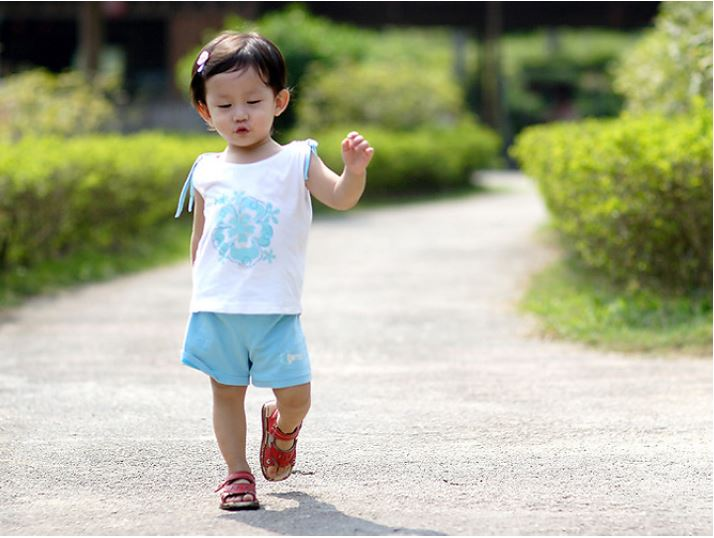
\includegraphics[width=0.4\linewidth]{pics/input}
	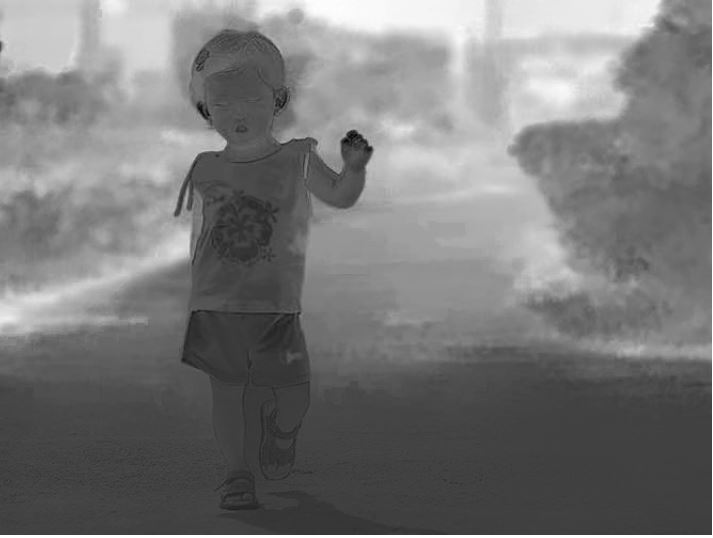
\includegraphics[width=0.4\linewidth]{pics/depth_map}
	\caption{Входное изображение и карта глубины}
	\label{fig:input}
\end{figure}

Сосредоточимся на более сложной проблеме восстановления относительной глубины из одного расфокусированного изображения, захваченного некалиброванной обычной камерой. Метод обратной диффузии~\cite{Proc} моделирует размытие дефокусировки в качестве процесса диффузии тепла и использует неоднородную диффузию тепла для оценки размытости размытия в краевых положениях. В отличие от этого, моделируем размытие дефокусировки как размытие 2D Gaussian. Входное изображение повторно размывается с использованием известного гауссовского размытия, и рассчитывается коэффициент градиента между входными и повторно размытыми изображениями. Величина размытия в краевых местоположениях может быть получена из отношения.

Рассмотрим эффективный метод оценки размытия, основанный на гауссовском градиентном соотношении, и показываем, что он устойчив к шуму, неточному расположению краев и помехам от соседних ребер. Без каких-либо изменений в камерах или при использовании дополнительного освещения наш метод позволяет получить карту глубины сцены, используя только одно расфокусированное изображение, снятое обычной камерой. Как показано (рисунок~\ref{fig:input}), этот метод может извлекать карту глубины сцены с довольно высокой степенью точности.


\subsection{Тестирование стабильности и качества алгоритма}

\begin{figure}[H]
	\centering
	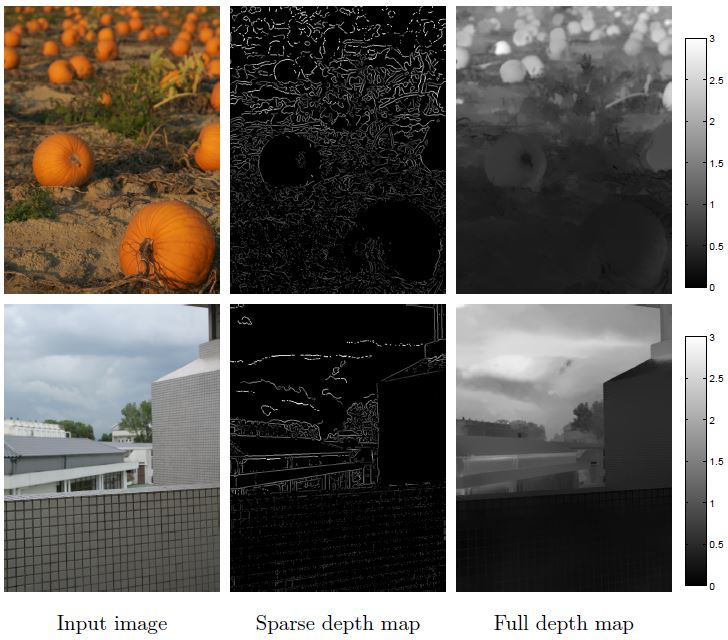
\includegraphics[width=0.7\linewidth]{pics/comparison}
	\caption{Восстановление глубины на реальных изображениях. Наш метод может работать как на сценах с непрерывной глубиной (изображение тыквы), так и на слоистой глубине (изображение здания) для получения карты глубины с довольно хорошей точностью.}
	\label{fig:comparison}
\end{figure}\

Как показано на рисунке~\ref{fig:comparison}, я тестирую наш метод на некоторых реальных изображениях. В изображении тыквы глубина сцены непрерывно изменяется от нижней к верхней части изображения. Оценочная карта глубины фиксирует непрерывное изменение глубины. В изображении здания сцена в основном содержит три слоя: стены, дом и небо. Наш метод позволяет создавать карты глубин, точно представляющие эти слои глубины. Как видно из результатов, наш метод позволяет точно восстановить глубину сцены из одного расфокусированного изображения. На рисунке~\ref{fig:flower} мы сравниваем наш метод с методом обратной диффузии~\cite{Proc}.

\begin{figure}[H]
	\centering
	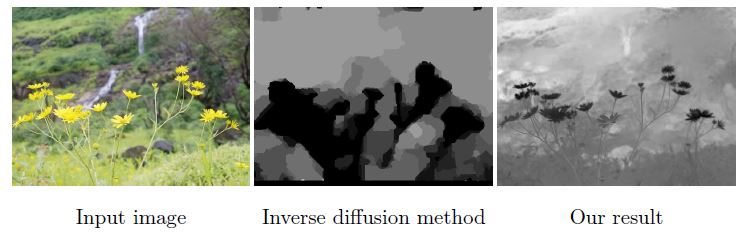
\includegraphics[width=1\linewidth]{pics/flower}
	\caption{Сравнение нашего метода с методом обратной диффузии, на примере цветка}
	\label{fig:flower}
\end{figure}\

Метод обратной диффузии создает грубую слоистую карту глубины. В результате этого цветочный слой плохо отделен фоновыми слоями и содержит некоторые оценки погрешности. Напротив, наш метод способен производить более точную и непрерывную карту глубины, а цветочный слой хорошо отделен фоновой травой и деревьями.